\chapter{\textbf{Конструкторский раздел}}

\hfill

Разрабатываемое программное обеспечения можно разделить на подзадачи:
\begin{itemize}
\item загружаемый модуль ядра;
\item приложение для шифрования файлов.
\end{itemize}

\section{\textbf{Перехват сообщений}}

\hfill

Для перехвата сообщений добавление нового USB устройства и удаление USB устройства необходимо в загружаемом модуле ядра разместить уведомитель, принимающий в качества параметра функцию обратного вызова нашей обработки данного события.

Для этого была создана следующая структура представленная в листинге \ref{lst:usb_notify}.

 \begin{lstlisting}[caption = Структура usb\_notify, label =  lst:usb_notify]
static struct notifier_block usb_notify = {
    .notifier_call = notify,
};
 \end{lstlisting}
 
 В этой структуре содержится указатель на прототип нашей функции обработки:

\textit{static int notify(struct notifier\_block *self, unsigned long action, void *dev)}

Для создания уведомителя передаем созданную структуру в функцию:

\textit{usb\_register\_notify(\&usb\_notify);}

Для удаления уведомителя передаем структуру в функцию:

\textit{usb\_unregister\_notify(\&usb\_notify);}

\section{\textbf{Хранение информации}}

\hfill

Для хранения информации о подключенных USB устройствах создадим структуру, листинг \ref{lst:our_usb_device}.

 \begin{lstlisting}[caption = Структура our\_usb\_device, label =  lst:our_usb_device]
typedef struct our_usb_device {
    struct usb_device_id dev_id;
    struct list_head list_node;
} our_usb_device_t;
 \end{lstlisting}
 
 Инициализируем список: \textit{LIST\_HEAD(connected\_devices);}

Для добавления нового подключенного устройства используется функция \ref{lst:add_usb},  для удаления -- \ref{lst:del_usb}.

\section{\textbf{Алгоритм работы функции-обработчика}}

На рисунке \ref{img:alg} представлен алгоритм работы функции обратного вызова добавления или удаления USB устройства.

\begin{figure}[H]
	\centering
	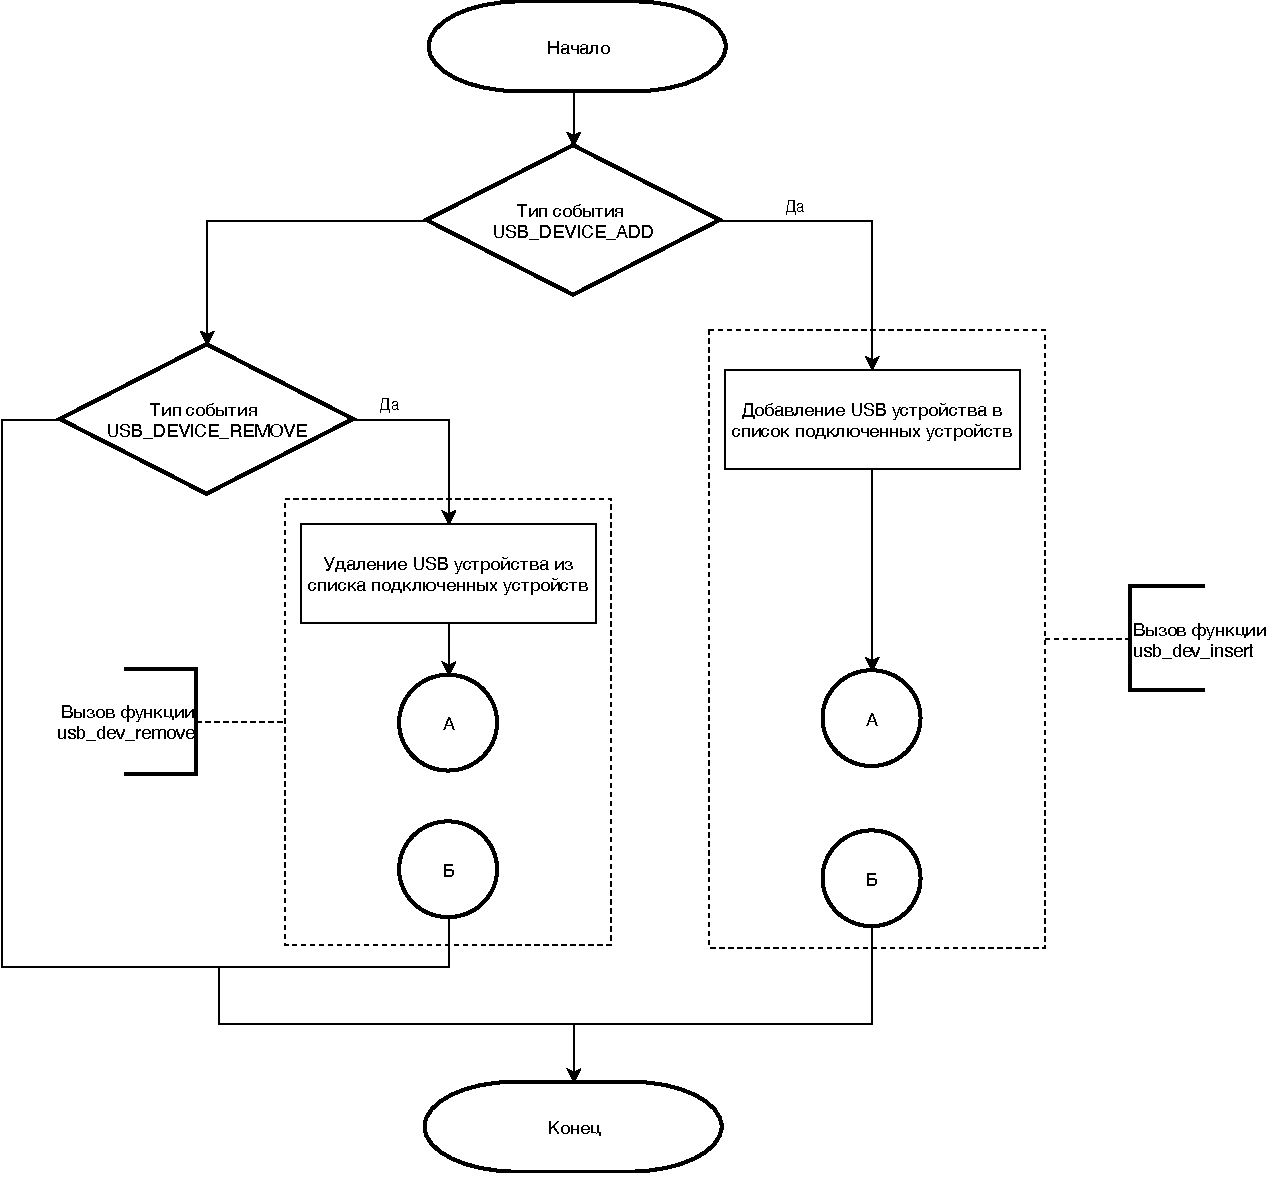
\includegraphics[scale=0.8]{alg1}
	\caption{Алгоритм работы функции-обработчика. }
	\label{img:alg}
\end{figure}

\begin{figure}[H]
	\centering
	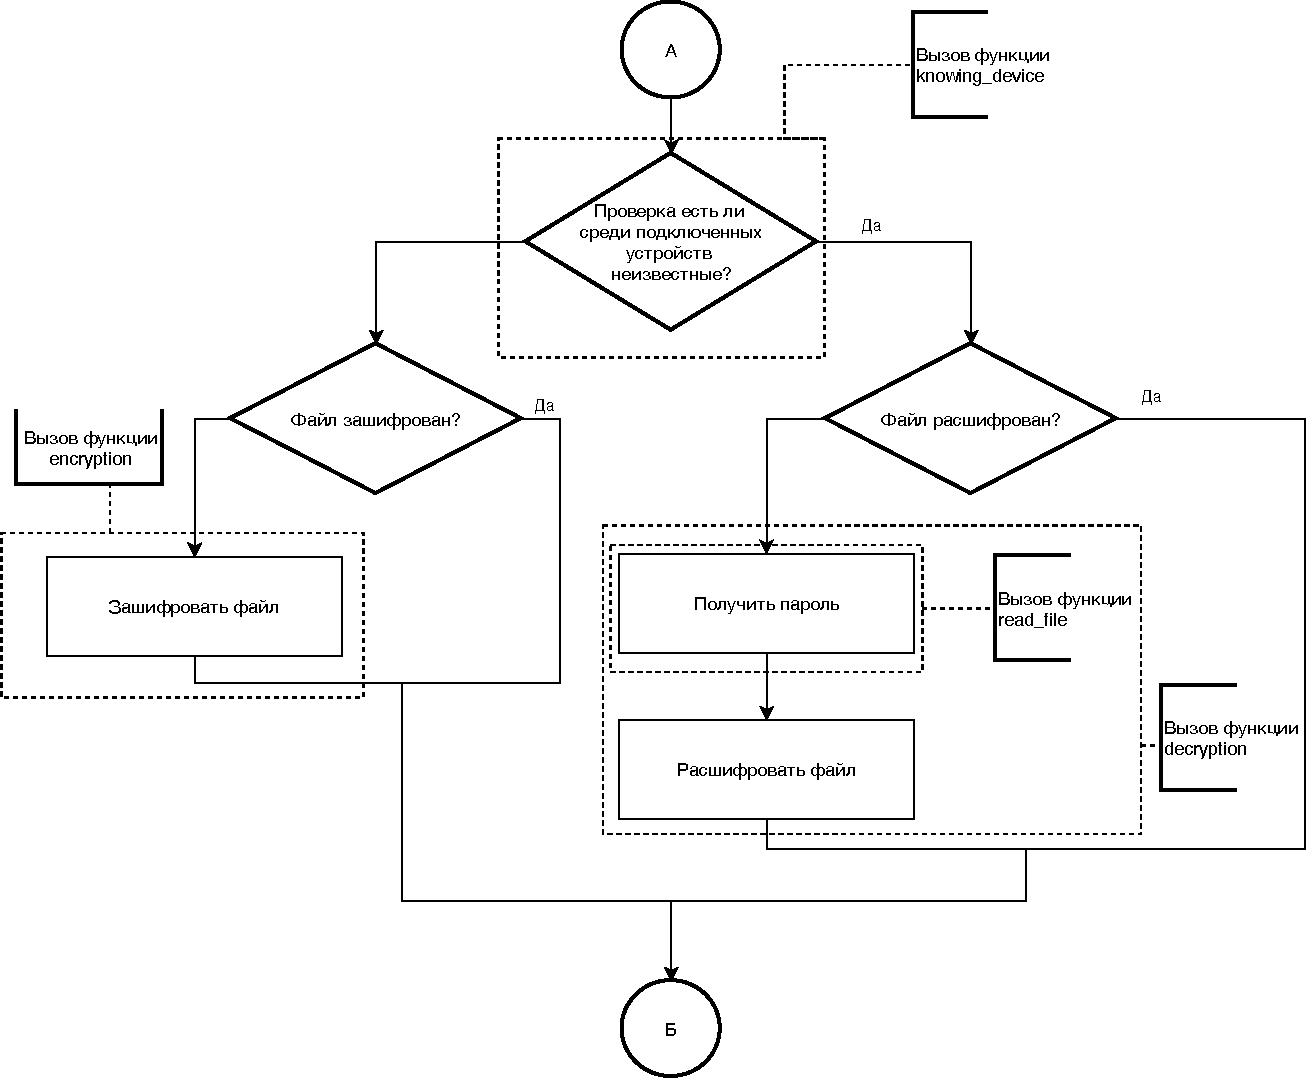
\includegraphics[scale=0.8]{alg2}
	\caption{Алгоритм работы функции-обработчика. }
	\label{img:alg1}
\end{figure}

\section{\textbf{Алгоритм шифрования файла}}

Для каждого файла из списка секретных.
 
\begin{enumerate}
\item[1. ] Побайтовое считывание символов из файла. 
\item[2. ] Применение операции XOR для данных с паролем. 
\item[3. ] Побайтовая запись символов в файл.  
\end{enumerate}


\section{\textbf{Вывод}}

\hfill

Структура программного обеспечения разработана, переход к реализации. 
